% Options for packages loaded elsewhere
\PassOptionsToPackage{unicode}{hyperref}
\PassOptionsToPackage{hyphens}{url}
%
\documentclass[
  12pt,
]{article}
\title{Hurricane Trends Along the East Coast}
\usepackage{etoolbox}
\makeatletter
\providecommand{\subtitle}[1]{% add subtitle to \maketitle
  \apptocmd{\@title}{\par {\large #1 \par}}{}{}
}
\makeatother
\subtitle{\url{https://github.com/elise-227/BoosBrantleyHusted_ENV872_EDA_FinalProject.git}}
\author{Elise Boos, Andrew Brantley, Kelsey Husted}
\date{}

\usepackage{amsmath,amssymb}
\usepackage{lmodern}
\usepackage{iftex}
\ifPDFTeX
  \usepackage[T1]{fontenc}
  \usepackage[utf8]{inputenc}
  \usepackage{textcomp} % provide euro and other symbols
\else % if luatex or xetex
  \usepackage{unicode-math}
  \defaultfontfeatures{Scale=MatchLowercase}
  \defaultfontfeatures[\rmfamily]{Ligatures=TeX,Scale=1}
  \setmainfont[]{Times New Roman}
\fi
% Use upquote if available, for straight quotes in verbatim environments
\IfFileExists{upquote.sty}{\usepackage{upquote}}{}
\IfFileExists{microtype.sty}{% use microtype if available
  \usepackage[]{microtype}
  \UseMicrotypeSet[protrusion]{basicmath} % disable protrusion for tt fonts
}{}
\makeatletter
\@ifundefined{KOMAClassName}{% if non-KOMA class
  \IfFileExists{parskip.sty}{%
    \usepackage{parskip}
  }{% else
    \setlength{\parindent}{0pt}
    \setlength{\parskip}{6pt plus 2pt minus 1pt}}
}{% if KOMA class
  \KOMAoptions{parskip=half}}
\makeatother
\usepackage{xcolor}
\IfFileExists{xurl.sty}{\usepackage{xurl}}{} % add URL line breaks if available
\IfFileExists{bookmark.sty}{\usepackage{bookmark}}{\usepackage{hyperref}}
\hypersetup{
  pdftitle={Hurricane Trends Along the East Coast},
  pdfauthor={Elise Boos, Andrew Brantley, Kelsey Husted},
  hidelinks,
  pdfcreator={LaTeX via pandoc}}
\urlstyle{same} % disable monospaced font for URLs
\usepackage[margin=2.54cm]{geometry}
\usepackage{longtable,booktabs,array}
\usepackage{calc} % for calculating minipage widths
% Correct order of tables after \paragraph or \subparagraph
\usepackage{etoolbox}
\makeatletter
\patchcmd\longtable{\par}{\if@noskipsec\mbox{}\fi\par}{}{}
\makeatother
% Allow footnotes in longtable head/foot
\IfFileExists{footnotehyper.sty}{\usepackage{footnotehyper}}{\usepackage{footnote}}
\makesavenoteenv{longtable}
\usepackage{graphicx}
\makeatletter
\def\maxwidth{\ifdim\Gin@nat@width>\linewidth\linewidth\else\Gin@nat@width\fi}
\def\maxheight{\ifdim\Gin@nat@height>\textheight\textheight\else\Gin@nat@height\fi}
\makeatother
% Scale images if necessary, so that they will not overflow the page
% margins by default, and it is still possible to overwrite the defaults
% using explicit options in \includegraphics[width, height, ...]{}
\setkeys{Gin}{width=\maxwidth,height=\maxheight,keepaspectratio}
% Set default figure placement to htbp
\makeatletter
\def\fps@figure{htbp}
\makeatother
\setlength{\emergencystretch}{3em} % prevent overfull lines
\providecommand{\tightlist}{%
  \setlength{\itemsep}{0pt}\setlength{\parskip}{0pt}}
\setcounter{secnumdepth}{-\maxdimen} % remove section numbering
\ifLuaTeX
  \usepackage{selnolig}  % disable illegal ligatures
\fi

\begin{document}
\maketitle

\newpage
\tableofcontents 
\newpage

\hypertarget{list-of-tables}{%
\subsection{List of Tables}\label{list-of-tables}}

\begin{itemize}
\tightlist
\item
  Table @ref(tab:table1): Data Structure
\item
  Table @ref(tab:table2): List of tau and p-values from time series
  analyses
\end{itemize}

\newpage

\hypertarget{list-of-figures}{%
\subsection{List of Figures}\label{list-of-figures}}

\begin{itemize}
\item
  Exploratory Analysis\\
  Figure @ref(fig:ex-an-FL): Florida Mean Daily Discharge During
  Hurricane Season\\
  Figure @ref(fig:ex-an-NC): North Carolina Mean Daily Discharge During
  Hurricane Season\\
  Figure @ref(fig:ex-NY): New York Mean Daily Discharge During Hurricane
  Season
\item
  Analysis\\
  Figure @ref(fig:NY-time-series-analysis): Decomposed Components of New
  York Time Series\\
  Figure @ref(fig:NY-time-series-analysis-continued): New York
  Non-Seasonal Daily Discharge During Hurricane Season\\
  Figure @ref(fig:NC-time-series-analysis): Decomposed Components of
  North Carolina Time Series\\
  Figure @ref(fig:NC-time-series-analysis-cont): North Carolina
  Non-Seasonal Daily Discharge During Hurricane Season\\
  Figure @ref(fig:FL-analysis-time-series): Decomposed Components of
  Florida Time Series\\
  Figure @ref(fig:FL-analysis-final-plot): Florida Non-Seasonal Daily
  Discharge During Hurricane Season\\
  Figure @ref(fig:combined-plot): Comparison Between Three Sites:
  Non-Seasonal Daily Discharge During Hurricane Season
\end{itemize}

\newpage
\listoffigures

\hypertarget{rationale-and-research-questions}{%
\section{Rationale and Research
Questions}\label{rationale-and-research-questions}}

Hurricanes are a serious natural disaster that affects millions each
year along the East Coast of the United States. Furthermore, hurricanes
create severe flooding, dangerous storm surges, and high winds that have
long-lasting and devastating consequences on many communities (Schmeltz
et al.~2013). Understanding how climate change influences the trends of
hurricanes will be informative for strategic planning to protect both
property and lives in the future (Mudd et al.~2014). For this analysis
we chose to look at discharge data in the vicinity of major rivers in
states spanning the East Coast of the US. The objective of the analysis
is to gain valuable insight on how locality and intensity of these
hurricanes may be changing over the past three decades.

Discharge data in Florida, North Carolina, and New York will be used to
gain a better understanding of how hurricane regimes change across the
entire span of the coast through time. Furthermore, the comparative
study will reveal if hurricanes are shifting poleward. Our central
research questions revolve around investigating any increasing trends in
discharge during the hurricane season (June-October) and where these
increasing trends are more intense.

\hypertarget{research-questions}{%
\section{Research Questions}\label{research-questions}}

\textbf{Question 1}: Has there been an overall increase in mean daily
discharge during the Atlantic hurricane season from 1990 - 2021?

\textbf{Question 2}: Has one portion of the East Coast of the US
experienced a disproportionate increase in hurricane activity, and its
associated discharge, compared to other portions commonly affected by
these hurricanes?

\textbf{Question 3}: Are the general locations of hurricanes shifting
towards the poles in the northern and/or southern hemisphere?

\newpage

\hypertarget{dataset-information}{%
\section{Dataset Information}\label{dataset-information}}

All datasets used in this analysis were downloaded from the United
States Geological Survey (USGS) website, specifically from historical
records of discharge data recorded by field dataloggers. The data was
obtained from three states varying in latitude along the East Coast
(i.e., Florida, North Carolina, and New York). Stream gage locations
were selected based on proximity to major river basins and vulnerable
counties susceptible to hurricane impacts. Additionally, gage locations
were specifically chosen with sufficient data, going back to at least
the 1990s. Similar timeline ranges for the datatsets ensures a time
series analysis that is comparable among all three sites. Discharge data
was the data type used in this analysis with all datasets having at
minimum daily recordings but some having recordings as often as every 30
minutes. The basic data structure is outlined below (Table
@ref(tab:table1)).

\begin{longtable}[]{@{}ll@{}}
\caption{Table summarizing the dataset structure}\tabularnewline
\toprule
Column Name & Description \\
\midrule
\endfirsthead
\toprule
Column Name & Description \\
\midrule
\endhead
Agency & USGS \\
SiteNumber & USGS gage number \\
MeanDischarge & Mean daily discharge (cfs) \\
Date & Date of collection \\
Month & Month of collection \\
\bottomrule
\end{longtable}

\newpage

\hypertarget{data-wrangling}{%
\section{Data Wrangling}\label{data-wrangling}}

Downloaded datasets included date/time and mean discharge (cfs) columns.
After the date column was properly classified as a date, unnecessary
columns were removed from the data frame. Next, the date column was
separated out to filter for years 1990-2021 and to filter for hurricane
months (June-October). The dataset was then saved into the processed
folder for each of the research locations. Missing data values were then
filled using a linear interpolation and then daily averages of discharge
were created in a new, clean column of daily means. After all fo these
steps were taken the data was considered to be wrangled and was then
ready for initial visualizations.

\newpage

\hypertarget{exploratory-analysis}{%
\section{Exploratory Analysis}\label{exploratory-analysis}}

The exploratory analysis of the data involved creating a map of the USGS
gage locations along the East Coast of the U.S. to orient individuals
towards the locality of the research. Also, the initial visualizations
of the discharge data for each research location-during hurricane
seasons-was included in the exploratory analysis from
\textasciitilde1990-2021. After the initial graphs displayed poorly
visualized data, a log scale was applied to the y-axis in order to
better present any noticeable trend that may be occurring. Comparing
differences between the intensity, frequency, and shifts in these
variables over time, permitted researchers to formulate predictions on
possible changes in each research location as well as any changes over
time. However, to fully understand these shifting trends, the following
time series analysis was conducted.

Below is a map of where each USGS gage site is located along the
Atlantic coast of the US.

\#\texttt{\{r\ map\ of\ locations,\ warning=FALSE,echo=FALSE\}\ \#site\_locations\ \textless{}-\ read.csv("../Data/Raw/Site\_locations.csv",\ stringsAsFactors\ =\ T)\ \#site\_locations.sf\ \textless{}-\ site\_locations\ \%\textgreater{}\%\ \#st\_as\_sf(coords\ =\ c(\textquotesingle{}Long\textquotesingle{},\textquotesingle{}Lat\textquotesingle{}),\ \#\ \ \ \ \ \ \ \ \ crs=4269)\ \#mapview(site\_locations.sf{[}1,{]},\ zcol\ =\ "Site.Name",\ col.regions\ =\ "deeppink1")\ +\ \#mapview(site\_locations.sf{[}2,{]},\ zcol\ =\ "Site.Name",\ col.regions\ =\ "turquoise4")\ +\ \#mapview(site\_locations.sf{[}3,{]},\ zcol\ =\ "Site.Name",\ col.regions\ =\ "forestgreen")\ \#}

Figure @ref(fig:ex-an-FL) is an initial plot of discharge within
hurricane months at the Florida location and shows a potential decrease
in discharge over time.

\begin{figure}

{\centering 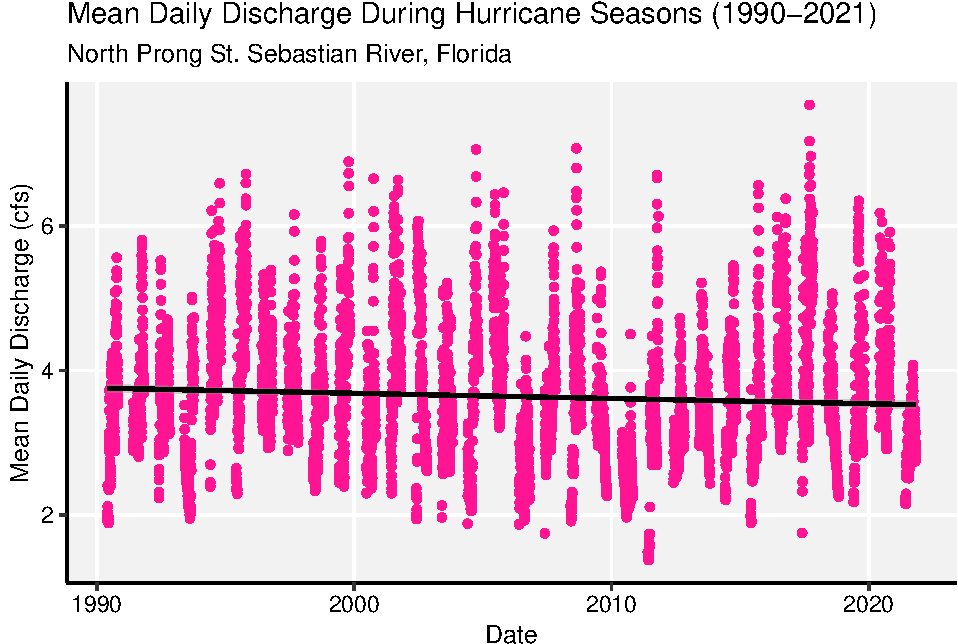
\includegraphics{BoosBrantleyHusted_ENV872_Project_files/figure-latex/ex-an-FL-1} 

}

\caption{Florida Discharge (cfs) 1990-2021}\label{fig:ex-an-FL}
\end{figure}

The following plot (Figure @ref(fig:ex-an-NC)) for the North Carolina
daily discharge dataset displays a potential increasing trend over time.

\begin{figure}

{\centering 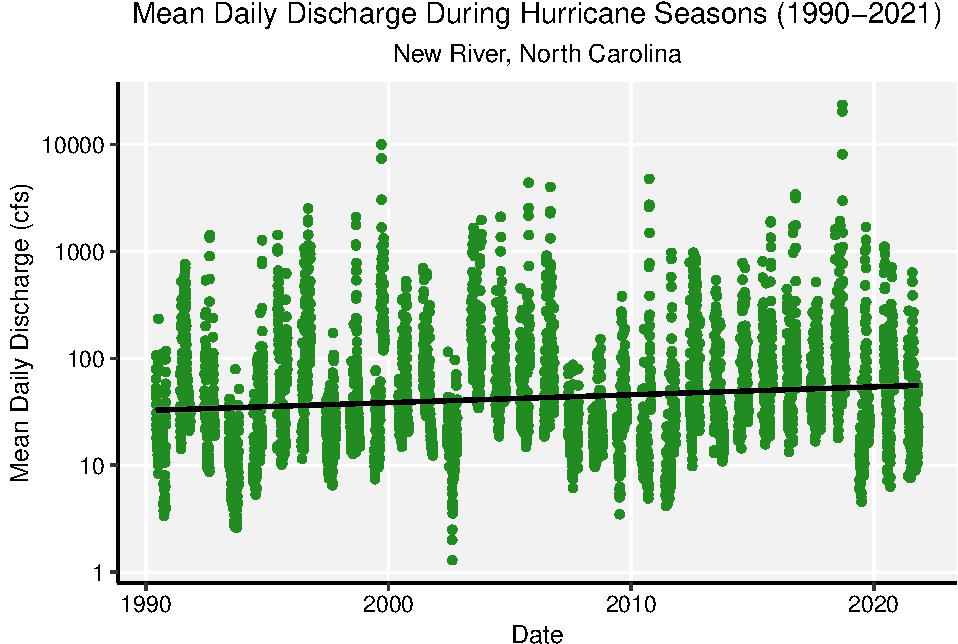
\includegraphics{BoosBrantleyHusted_ENV872_Project_files/figure-latex/ex-an-NC-1} 

}

\caption{North Carolina Discharge (cfs) 1990-2021}\label{fig:ex-an-NC}
\end{figure}

The following Figure @ref(fig:ex-NY) for the New York daily discharge
dataset displays a potential increasing trend over time.

\begin{figure}

{\centering 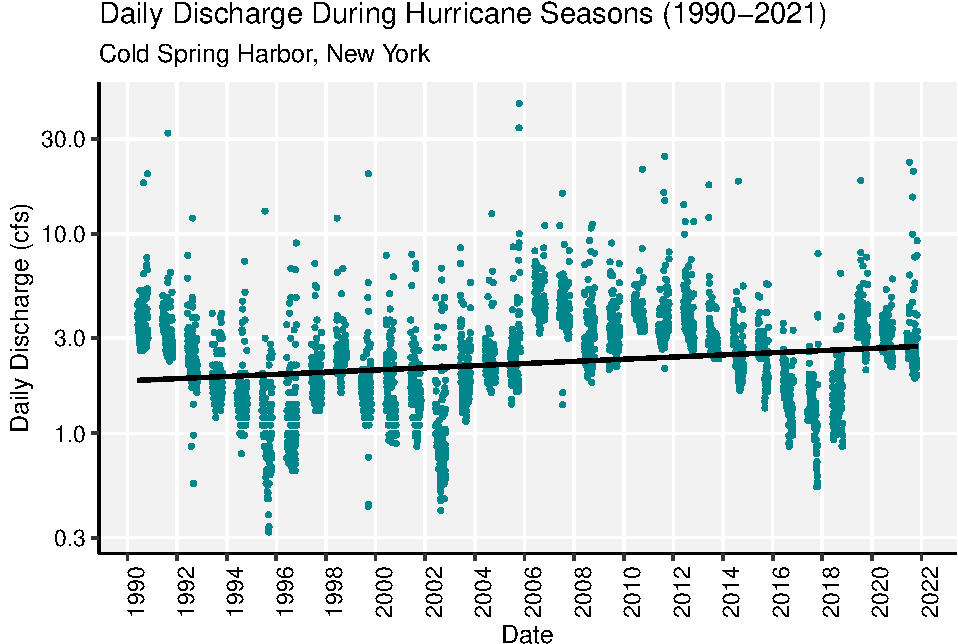
\includegraphics{BoosBrantleyHusted_ENV872_Project_files/figure-latex/ex-NY-1} 

}

\caption{New York Discharge (cfs) 1990-2021}\label{fig:ex-NY}
\end{figure}

\newpage

\hypertarget{analysis}{%
\section{Analysis}\label{analysis}}

The analysis of these datasets centers on creating time series objects
of the discharge data. These time series objects are then decomposed to
analyze the trend, seasonality, and remainder for the data values. New
dataframes were then created with these three aspects of the time
series. Within these dataframes, the trend and remainder values for each
data point were combined to create a ``non-seasonal'' discharge value in
order to better understand the actual changes in hurricane intensity and
frequency during the hurricane season.

These non-seasonal values were then used to create another time series
object which was graphed to visualize potential trends that may be
occurring in the data as well as the spread of the discharge values. The
spread of the discharge values indicates differences in discharge which
is a proxy for hurricane intensity. To analyze trends statistically,
rather than visually, a Mann Kendall test was performed. The Mann
Kendall test produced a tau value which indicated whether the trend was
increasing or decreasing. The tau values were compared across all three
research locations in addition to p-values which displayed statistical
significance of the results.

\hypertarget{new-york-analysis}{%
\subsubsection{New York Analysis}\label{new-york-analysis}}

The following plot displays the decomposed daily discharge components of
the time series run on the New York dataset during hurricane season
(Figure @ref(fig:NY-time-series-analysis)).

\begin{figure}

{\centering 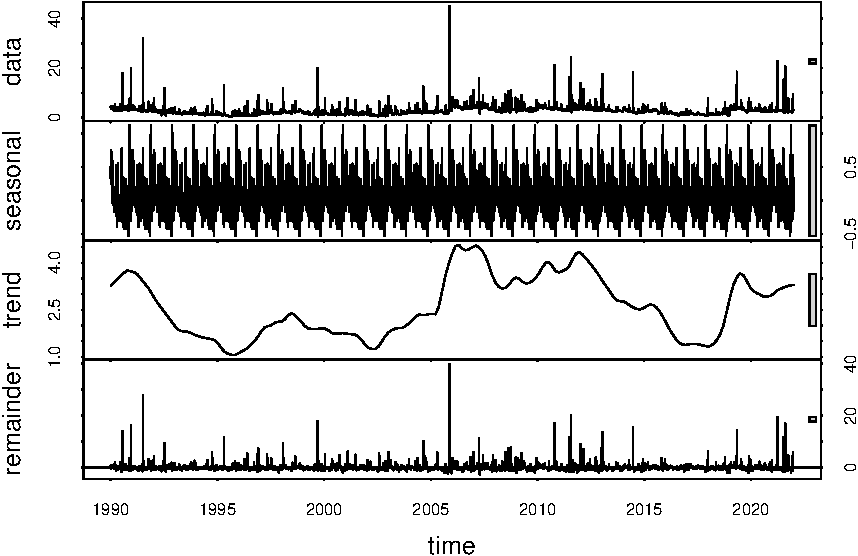
\includegraphics{BoosBrantleyHusted_ENV872_Project_files/figure-latex/NY-time-series-analysis-1} 

}

\caption{Decomposed Components of the New York Discharge Time Series}\label{fig:NY-time-series-analysis}
\end{figure}

\begin{verbatim}
## tau = 0.13, 2-sided pvalue =< 2.22e-16
\end{verbatim}

The Mann Kendall analysis performed on the New York non-seasonal time
series produced a tau value of 0.13 with a p-value of less than 0.05. As
a result, the data displays a significant, increasing trend for New
York.

The plot below displays the non-seasonal daily discharge data in the New
York time series which was produced by removing the seasonal component
from the time series (Figure
@ref(fig:NY-time-series-analysis-continued)).

\begin{figure}

{\centering 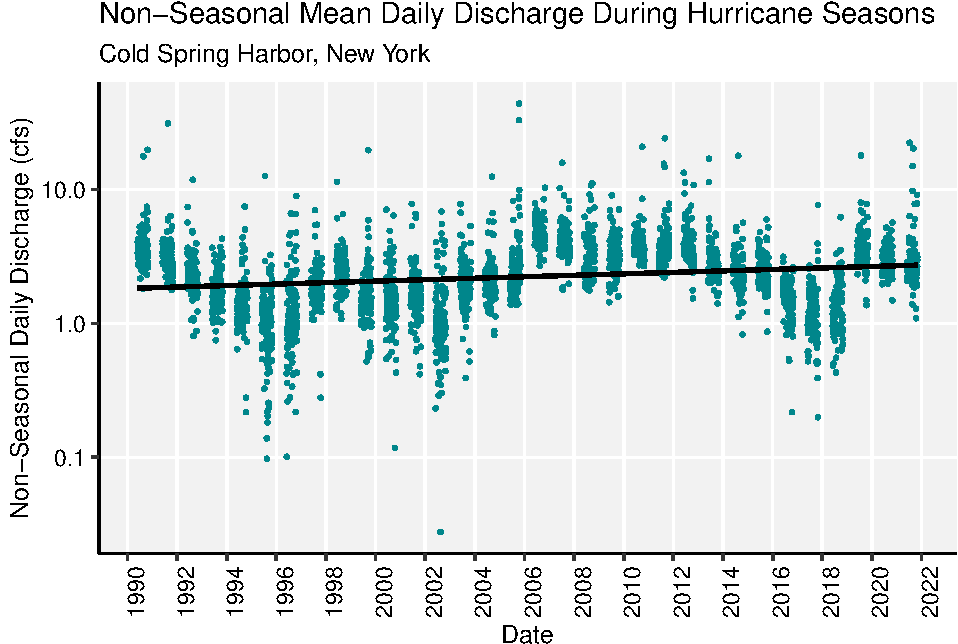
\includegraphics{BoosBrantleyHusted_ENV872_Project_files/figure-latex/NY-time-series-analysis-continued-1} 

}

\caption{Nonseasonal Data from the New York Discharge Time Series}\label{fig:NY-time-series-analysis-continued}
\end{figure}

\hypertarget{north-carolina-analysis}{%
\subsubsection{North Carolina Analysis}\label{north-carolina-analysis}}

\begin{figure}

{\centering 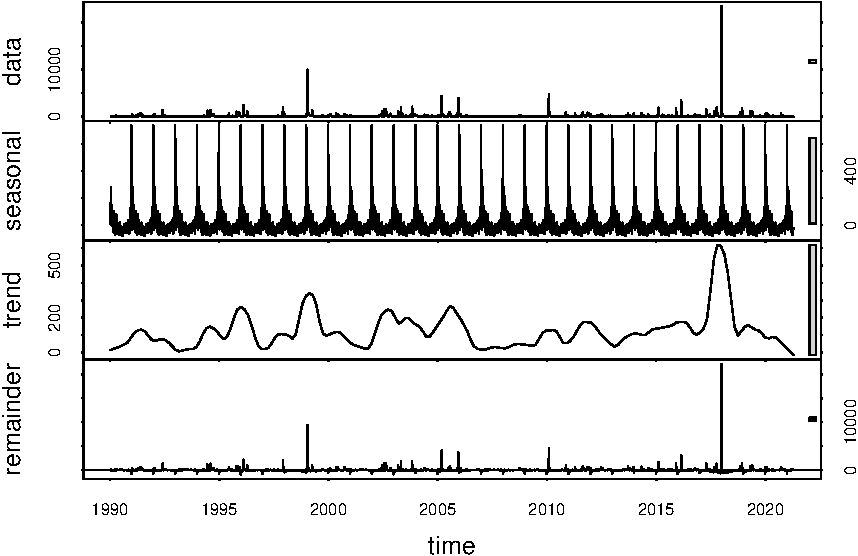
\includegraphics{BoosBrantleyHusted_ENV872_Project_files/figure-latex/NC-time-series-analysis-1} 

}

\caption{Decomposed Components of the North Carolina Discharge Time Series}\label{fig:NC-time-series-analysis}
\end{figure}

\begin{verbatim}
## tau = 0.0572, 2-sided pvalue =< 2.22e-16
\end{verbatim}

Above is the decomposed time series of the North Carolina discharge data
during hurricane months (Figure @ref(fig:NC-time-series-analysis)). The
Mann Kendall Test yielded a tau value of 0.0572 and a 2-sided p value of
=\textless{} 2.22e-16.

\begin{figure}

{\centering 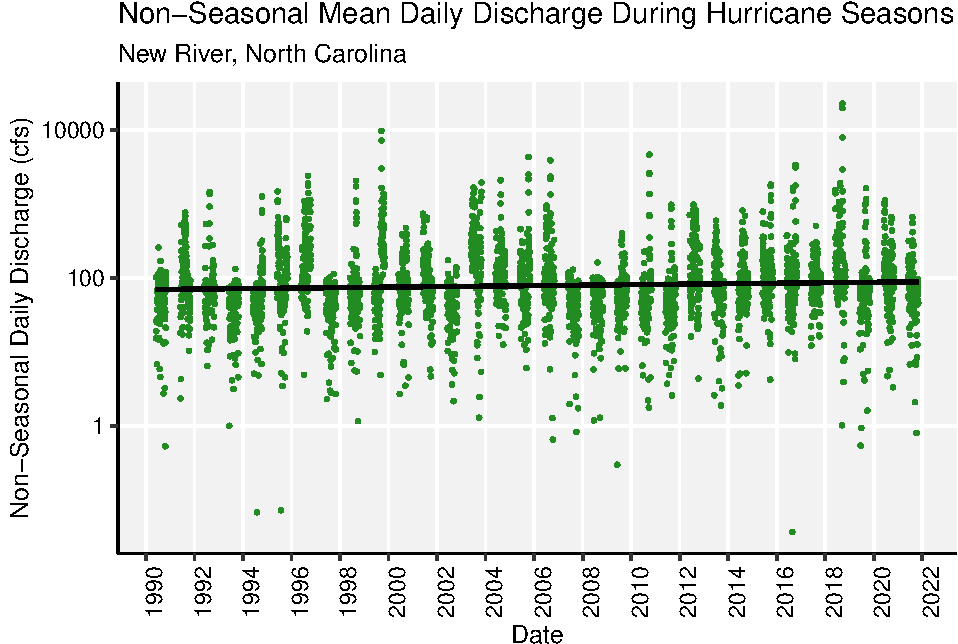
\includegraphics{BoosBrantleyHusted_ENV872_Project_files/figure-latex/NC-time-series-analysis-cont-1} 

}

\caption{Nonseasonal Data from the North Carolina Discharge Time Series}\label{fig:NC-time-series-analysis-cont}
\end{figure}

The plot above displays the non-seasonal data in the North Carolina time
series which was produced by removing the seasonal component from the
time series (Figure @ref(fig:NC-time-series-analysis)).

\hypertarget{florida-analysis}{%
\subsubsection{Florida Analysis}\label{florida-analysis}}

Seen below is the decomposed time series of the Florida discharge data
during hurricane months (Figure @ref(fig:FL-anlaysis-time-series)).

\begin{figure}

{\centering 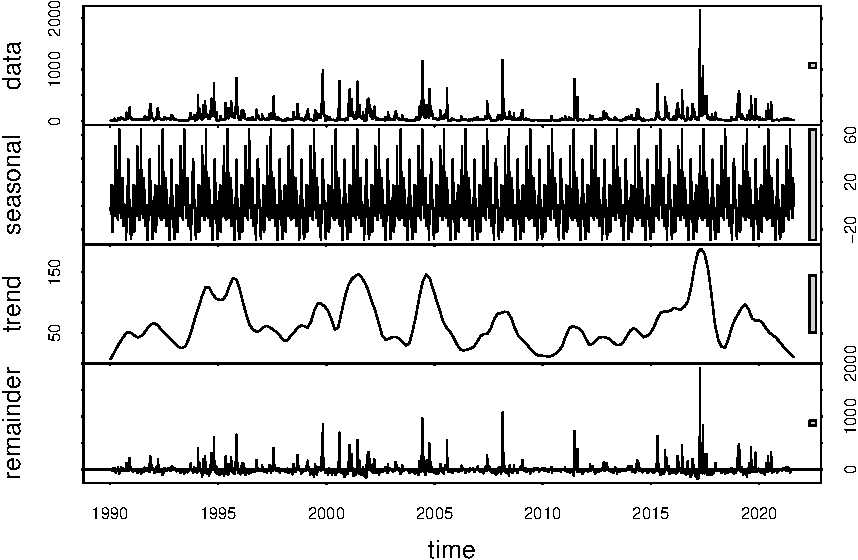
\includegraphics{BoosBrantleyHusted_ENV872_Project_files/figure-latex/FL-analysis-time-series-1} 

}

\caption{Decomposed plot of Florida discharge time series}\label{fig:FL-analysis-time-series}
\end{figure}

\begin{verbatim}
## tau = -0.0516, 2-sided pvalue =7.7953e-08
\end{verbatim}

From running a MannKendall nonseasonal trend analysis on the Florida
discharge data set there is a significant overall decline in discharge
over time with a tau value of -0.0516 (p = 7.7953e-08). Below this trend
is visualized in a plot of the non-seasonal time series of Florida
discharge with the significant decreasing trend shown with the black
line (Figure @ref(fig:FL-analysis-final-plot)).

\begin{figure}

{\centering 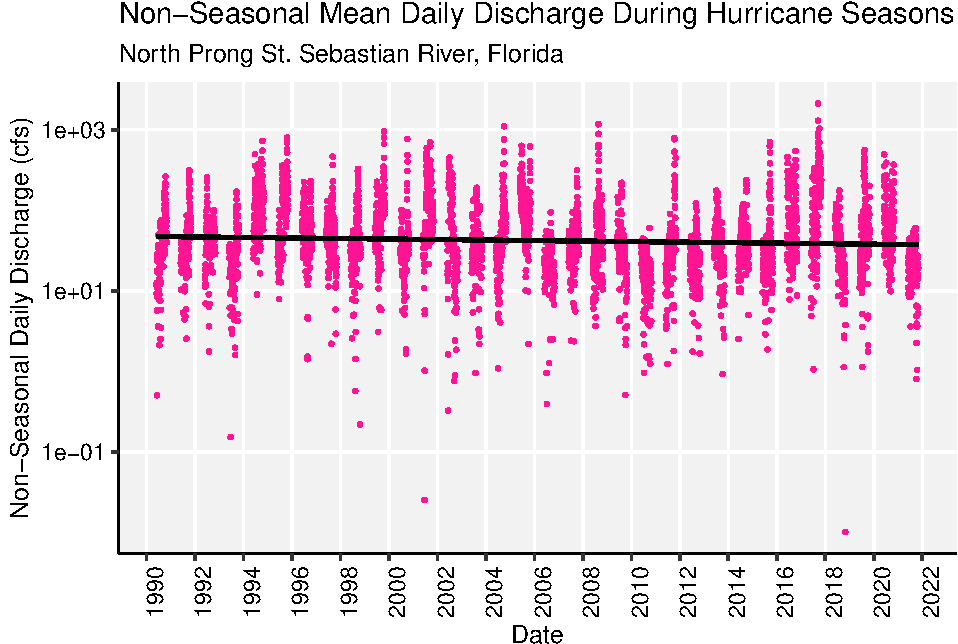
\includegraphics{BoosBrantleyHusted_ENV872_Project_files/figure-latex/FL-analysis-final-plot-1} 

}

\caption{Plot of nonseasonal time series of Florida discharge and overall trend}\label{fig:FL-analysis-final-plot}
\end{figure}

\hypertarget{comparison-between-sites}{%
\subsubsection{Comparison between
Sites}\label{comparison-between-sites}}

Each of the locations non-seasonal time series and trends are visualized
and compared in the figure below (Figure @ref(fig:combined-plot)). The
color patterns are the same as above with Florida in pink, North
Carolina in green, and New York in turquoise.

\begin{figure}

{\centering 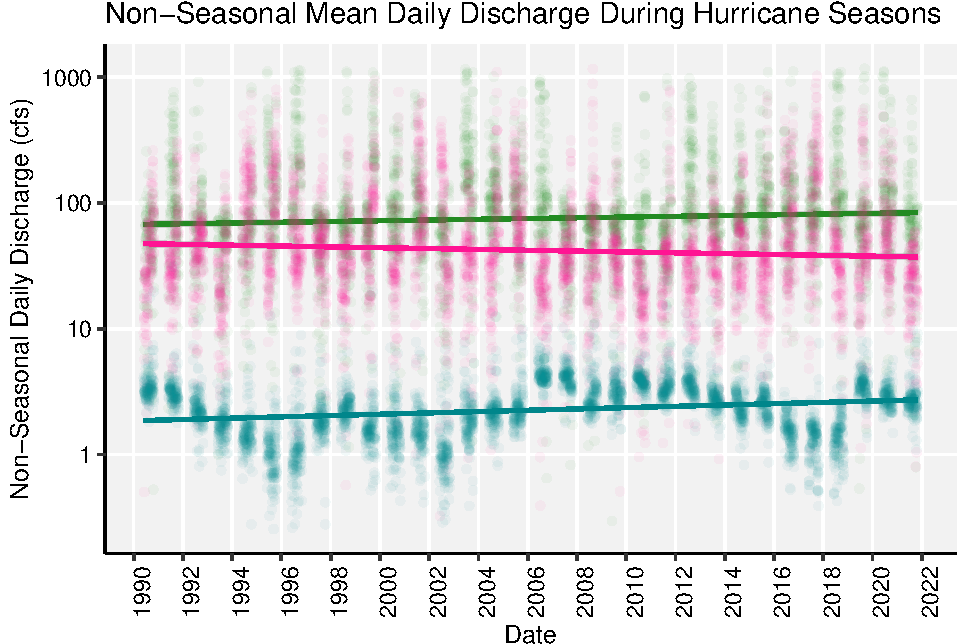
\includegraphics{BoosBrantleyHusted_ENV872_Project_files/figure-latex/combined-plot-1} 

}

\caption{Non-Seasonal Discharge Plot for all Gage Sites (cfs)}\label{fig:combined-plot}
\end{figure}

From this visual we can see that New York and North Carolina are seeing
upward trends while Florida is seeing a downward trend in discharge.
Also the overall discharge in New York is less than that of Florida and
North Carolina.

\newpage

\hypertarget{summary-and-conclusions}{%
\section{Summary and Conclusions}\label{summary-and-conclusions}}

A poleward hurricane trend is apparent based on the daily discharge
values associated with hurricane months across the East Coast of the
U.S. Although discharge is noticeably greater in Florida and North
Carolina, hurricane discharge trends are increasing in New York and
North Carolina while the last 30 years yielded a slightly decreasing
trend in Florida (Table @ref(tab:table2)). The effect of poleward
hurricane movement with increasing hurricane frequency/intensity could
potentially lead to exacerbated natural disasters in northern states of
the U.S. Large urban centers such as New York City are not equipped to
handle such severe rain events. Given the substantial amount of
impervious surface cover attributed to urbanization, future disastrous
flooding events are inevitable (Coch 2015). Further research on the
analysis could possibly include more sites along the East Coast to
better comprehend the trends that may be occurring in terms of where
hurricanes are becoming more/less frequent and intense.

\begin{longtable}[]{@{}lrl@{}}
\caption{List of tau values and p-values from non-seasonal time series
analyses.}\tabularnewline
\toprule
State & Tau value & P-value \\
\midrule
\endfirsthead
\toprule
State & Tau value & P-value \\
\midrule
\endhead
New York & 0.1300 & =\textless{} 2.22e-16 \\
North Carolina & 0.0572 & =\textless{} 2.22e-16 \\
Florida & -0.0516 & 7.7953e-08 \\
\bottomrule
\end{longtable}

\newpage

\hypertarget{references}{%
\section{References}\label{references}}

Coch, N. K. 2015. Unique vulnerability of the New York--New Jersey
metropolitan area to hurricane destruction. Journal of Coastal Research
31:196--212. Mudd, L., Y. Wang, C. Letchford, and D. Rosowsky. 2014.
Assessing climate change impact on the US East Coast hurricane hazard:
temperature, frequency, and track. Natural Hazards Review 15:4014001.
Schmeltz, M. T., S. K. González, L. Fuentes, A. Kwan, A.
Ortega-Williams, and L. P. Cowan. 2013. Lessons from hurricane sandy: a
community response in Brooklyn, New York. Journal of urban health
90:799--809.

\end{document}
